%%%%%%%%%%%%%%%%%%%%%%%%%%%%%%%%%%%%%%%%%%%%%%%%%%%%%%%%%%%%%%%
%
% Edit your LaTeX on the left, and it gets compiled for you on 
% the right. If you give someone the link to this page, they 
% can edit at the same time. See the help menu above for more 
% info. Enjoy!
%
%%%%%%%%%%%%%%%%%%%%%%%%%%%%%%%%%%%%%%%%%%%%%%%%%%%%%%%%%%%%%%%
\documentclass[11pt]{article}
\usepackage{fancyhdr}
\usepackage{graphicx}
\usepackage{amssymb}
\usepackage{epstopdf}
\usepackage{amsmath} 	
\usepackage{amssymb}
\usepackage{cite}
\usepackage{multirow}
\usepackage{wrapfig}
\usepackage{subfigure}
\usepackage{todonotes}
\usepackage{listings}
\usepackage[colorlinks=true, linkcolor=black,citecolor=black,urlcolor=blue]{hyperref}
\bibliographystyle{IEEEtran}
\DeclareGraphicsRule{.tif}{png}{.png}{`convert #1 `dirname #1`/`basename #1 .tif`.png}

%---------------- Letter Paper --------------------%
% be sure to change in document class too
\textwidth = 6.5 in
\textheight = 8.6 in
\oddsidemargin = 0.0 in
\evensidemargin = 0.0 in
\topmargin = 0.0 in
\headheight = 0.0 in
\headsep = 0.2in
\parskip = 0.2in
\parindent = 0.0in


\begin{document}
\thispagestyle{empty}
\begin{center}
\vspace*{1.5in}
{\LARGE \textbf{PROJECT TITLE}} %<---- Insert your project title here

{\Large MCHE 201: Introduction to Mechanical Design\\ \vspace*{0.1in} Spring 2015}

\vspace*{2.5in}

% author names and CLIDS
\begin{figure}[!h]
\begin{minipage}{0.45\textwidth}
\begin{center}
Author 1 \\
Department of Mechanical Engineering\\
University of Louisiana at Lafayette\\
Lafayette, LA 70504\\
{\tt CLID1@louisiana.edu}
\end{center}
\end{minipage}
\hspace{0.08\textwidth}
\begin{minipage}{0.45\textwidth}
\begin{center}
Author 2 \\
Department of Mechanical Engineering\\
University of Louisiana at Lafayette\\
Lafayette, LA 70504\\
\tt{CLID2@louisiana.edu}
\end{center}
\end{minipage}
\end{figure}
%
\vspace{0.2in}
\begin{figure}[!h]
\begin{minipage}{0.45\textwidth}
\begin{center}
Author 3 \\
Department of Mechanical Engineering\\
University of Louisiana at Lafayette\\
Lafayette, LA 70504\\
{\tt CLID3@louisiana.edu}
\end{center}
\end{minipage}
\hspace{0.08\textwidth}
\begin{minipage}{0.45\textwidth}
\begin{center}
Author 4 \\
Department of Mechanical Engineering\\
University of Louisiana at Lafayette\\
Lafayette, LA 70504\\
\tt{CLID4@louisiana.edu}
\end{center}
\end{minipage}
\end{figure}

\end{center}

\newpage
\thispagestyle{empty}
\begin{abstract}
\vspace{-0.2in}
Aliquam aliquet, est a ullamcorper condimentum, tellus nulla fringilla elit, a iaculis nulla turpis sed wisi. Fusce volutpat. Etiam sodales ante id nunc. Proin ornare dignissim lacus. Nunc porttitor nunc a sem. Sed sollicitudin velit eu magna. Aliquam erat volutpat. Vivamus ornare est non wisi. Proin vel quam. Vivamus egestas. Nunc tempor diam vehicula mauris. Nullam sapien eros, facilisis vel, eleifend non, auctor dapibus, pede. Ut nulla. Vivamus bibendum, nulla ut congue fringilla, lorem ipsum ultricies risus, ut rutrum velit tortor vel purus. In hac habitasse platea dictumst. Duis fermentum, metus sed congue gravida, arcu dui ornare urna, ut imperdiet enim odio dignissim ipsum. Nulla facilisi.
\end{abstract} 

\newpage
\setcounter{page}{1} % reset the page counter, so it begins with the page of the introduction section
%%%%%%%%%%%%%%%%%%%%%%%%%%%%%%%%%%%%%%%%%%%%%%%%%%%%%%%%%%%%%%%%
%%%%%%%%%%%%%%%%%%%%%%%%%%%%%%%%%%%%%%%%%%%%%%%%%%%%%%%%%%%%%%%%
\section{Introduction}
\label{sec:intro}
\vspace{-0.2in}
%
This is the introduction section\ldots Aliquam aliquet, est a ullamcorper condimentum, tellus nulla fringilla elit, a iaculis nulla turpis sed wisi. Fusce volutpat. Etiam sodales ante id nunc. Proin ornare dignissim lacus. Nunc porttitor nunc a sem. Sed sollicitudin velit eu magna. Aliquam erat volutpat. Vivamus ornare est non wisi. Proin vel quam. Vivamus egestas. Nunc tempor diam vehicula mauris. Nullam sapien eros, facilisis vel, eleifend non, auctor dapibus, pede. Ut nulla. Vivamus bibendum, nulla ut congue fringilla, lorem ipsum ultricies risus, ut rutrum velit tortor vel purus. In hac habitasse platea dictumst. Duis fermentum, metus sed congue gravida, arcu dui ornare urna, ut imperdiet enim odio dignissim ipsum. Nulla facilisi. 

Aliquam aliquet, est a ullamcorper condimentum, tellus nulla fringilla elit, a iaculis nulla turpis sed wisi. Fusce volutpat. Etiam sodales ante id nunc. Proin ornare dignissim lacus. Nunc porttitor nunc a sem. Sed sollicitudin velit eu magna. Aliquam erat volutpat. Vivamus ornare est non wisi. Proin vel quam. Vivamus egestas. Nunc tempor diam vehicula mauris. Nullam sapien eros, facilisis vel, eleifend non, auctor dapibus, pede. Ut nulla. Vivamus bibendum, nulla ut congue fringilla, lorem ipsum ultricies risus, ut rutrum velit tortor vel purus. In hac habitasse platea dictumst. Duis fermentum, metus sed congue gravida, arcu dui ornare urna, ut imperdiet enim odio dignissim ipsum. Nulla facilisi. 

%%%%%%%%%%%%%%%%%%%%%%%%%%%%%%%%%%%%%%%%%%%%%%%%%%%%%%%%%%%%%%%%
%%%%%%%%%%%%%%%%%%%%%%%%%%%%%%%%%%%%%%%%%%%%%%%%%%%%%%%%%%%%%%%%
\section{Section 2}
\label{sec:section_2_label}
\vspace{-0.2in}
%
Aliquam aliquet, est a ullamcorper condimentum, tellus nulla fringilla elit, a iaculis nulla turpis sed wisi. Fusce volutpat. Etiam sodales ante id nunc. Proin ornare dignissim lacus. Nunc porttitor nunc a sem. Sed sollicitudin velit eu magna. Aliquam erat volutpat. Vivamus ornare est non wisi. Proin vel quam. Vivamus egestas. Nunc tempor diam vehicula mauris. 

Nunc tempor diam vehicula mauris. Nullam sapien eros, facilisis vel, eleifend non, auctor dapibus, pede. Ut nulla. Vivamus bibendum, nulla ut congue fringilla, lorem ipsum ultricies risus, ut rutrum velit tortor vel purus. In hac habitasse platea dictumst. Duis fermentum, metus sed congue gravida, arcu dui ornare urna, ut imperdiet enim odio dignissim ipsum. Nulla facilisi. 


%%%%%%%%%%%%%%%%%%%%%%%%%%%%%%%%%%%%%%%%%%%%%%%%%%%%%%%%%%%%%%%%
\subsection{Equations}
\label{sec:subsection_label}
\vspace{-0.2in}
%
Equations numbering and formatting is also handled nicely by \LaTeX. An example equation is shown in (\ref{eqn:example}).

%
\begin{equation}
\ddot{x}_1 = \frac{1}{m}\left(-k x_1 - c\dot{x}_1 + F\right)
\label{eqn:example}
\end{equation}
%
The next equation is numbered automatically, as shown by (\ref{eqn:example2}).
%
\begin{equation}
\ddot{\theta} + \frac{g}{l}\theta = 0
\label{eqn:example2}
\end{equation}
%
Aliquam aliquet, est a ullamcorper condimentum, tellus nulla fringilla elit, a iaculis nulla turpis sed wisi. Fusce volutpat. Etiam sodales ante id nunc. Proin ornare dignissim lacus. Nunc porttitor nunc a sem. Sed sollicitudin velit eu magna. Aliquam erat volutpat. Vivamus ornare est non wisi. Proin vel quam. Vivamus egestas. 


%%%%%%%%%%%%%%%%%%%%%%%%%%%%%%%%%%%%%%%%%%%%%%%%%%%%%%%%%%%%%%%%
\subsection{Using Figures}
\label{sec:using_figures}
\vspace{-0.2in}
%
The experimental platform is shown in Figure \ref{fig:cherrypicker_labeled}. \LaTeX will handle numbering the figures in the order that they appear and inserting a properly formatted caption. 
If the figure file is not in the same folder as your \LaTeX document, then you need to specify the relative path to it. The figure environment is very powerful and customizable. A more thorough review of using figures in \LaTeX can be found at: 

\hspace{0.25in}\url{http://en.wikibooks.org/wiki/LaTeX/Floats,_Figures_and_Captions}
%

% This is the code block that includes the figure.
\begin{figure}[tbp]
\begin{center}
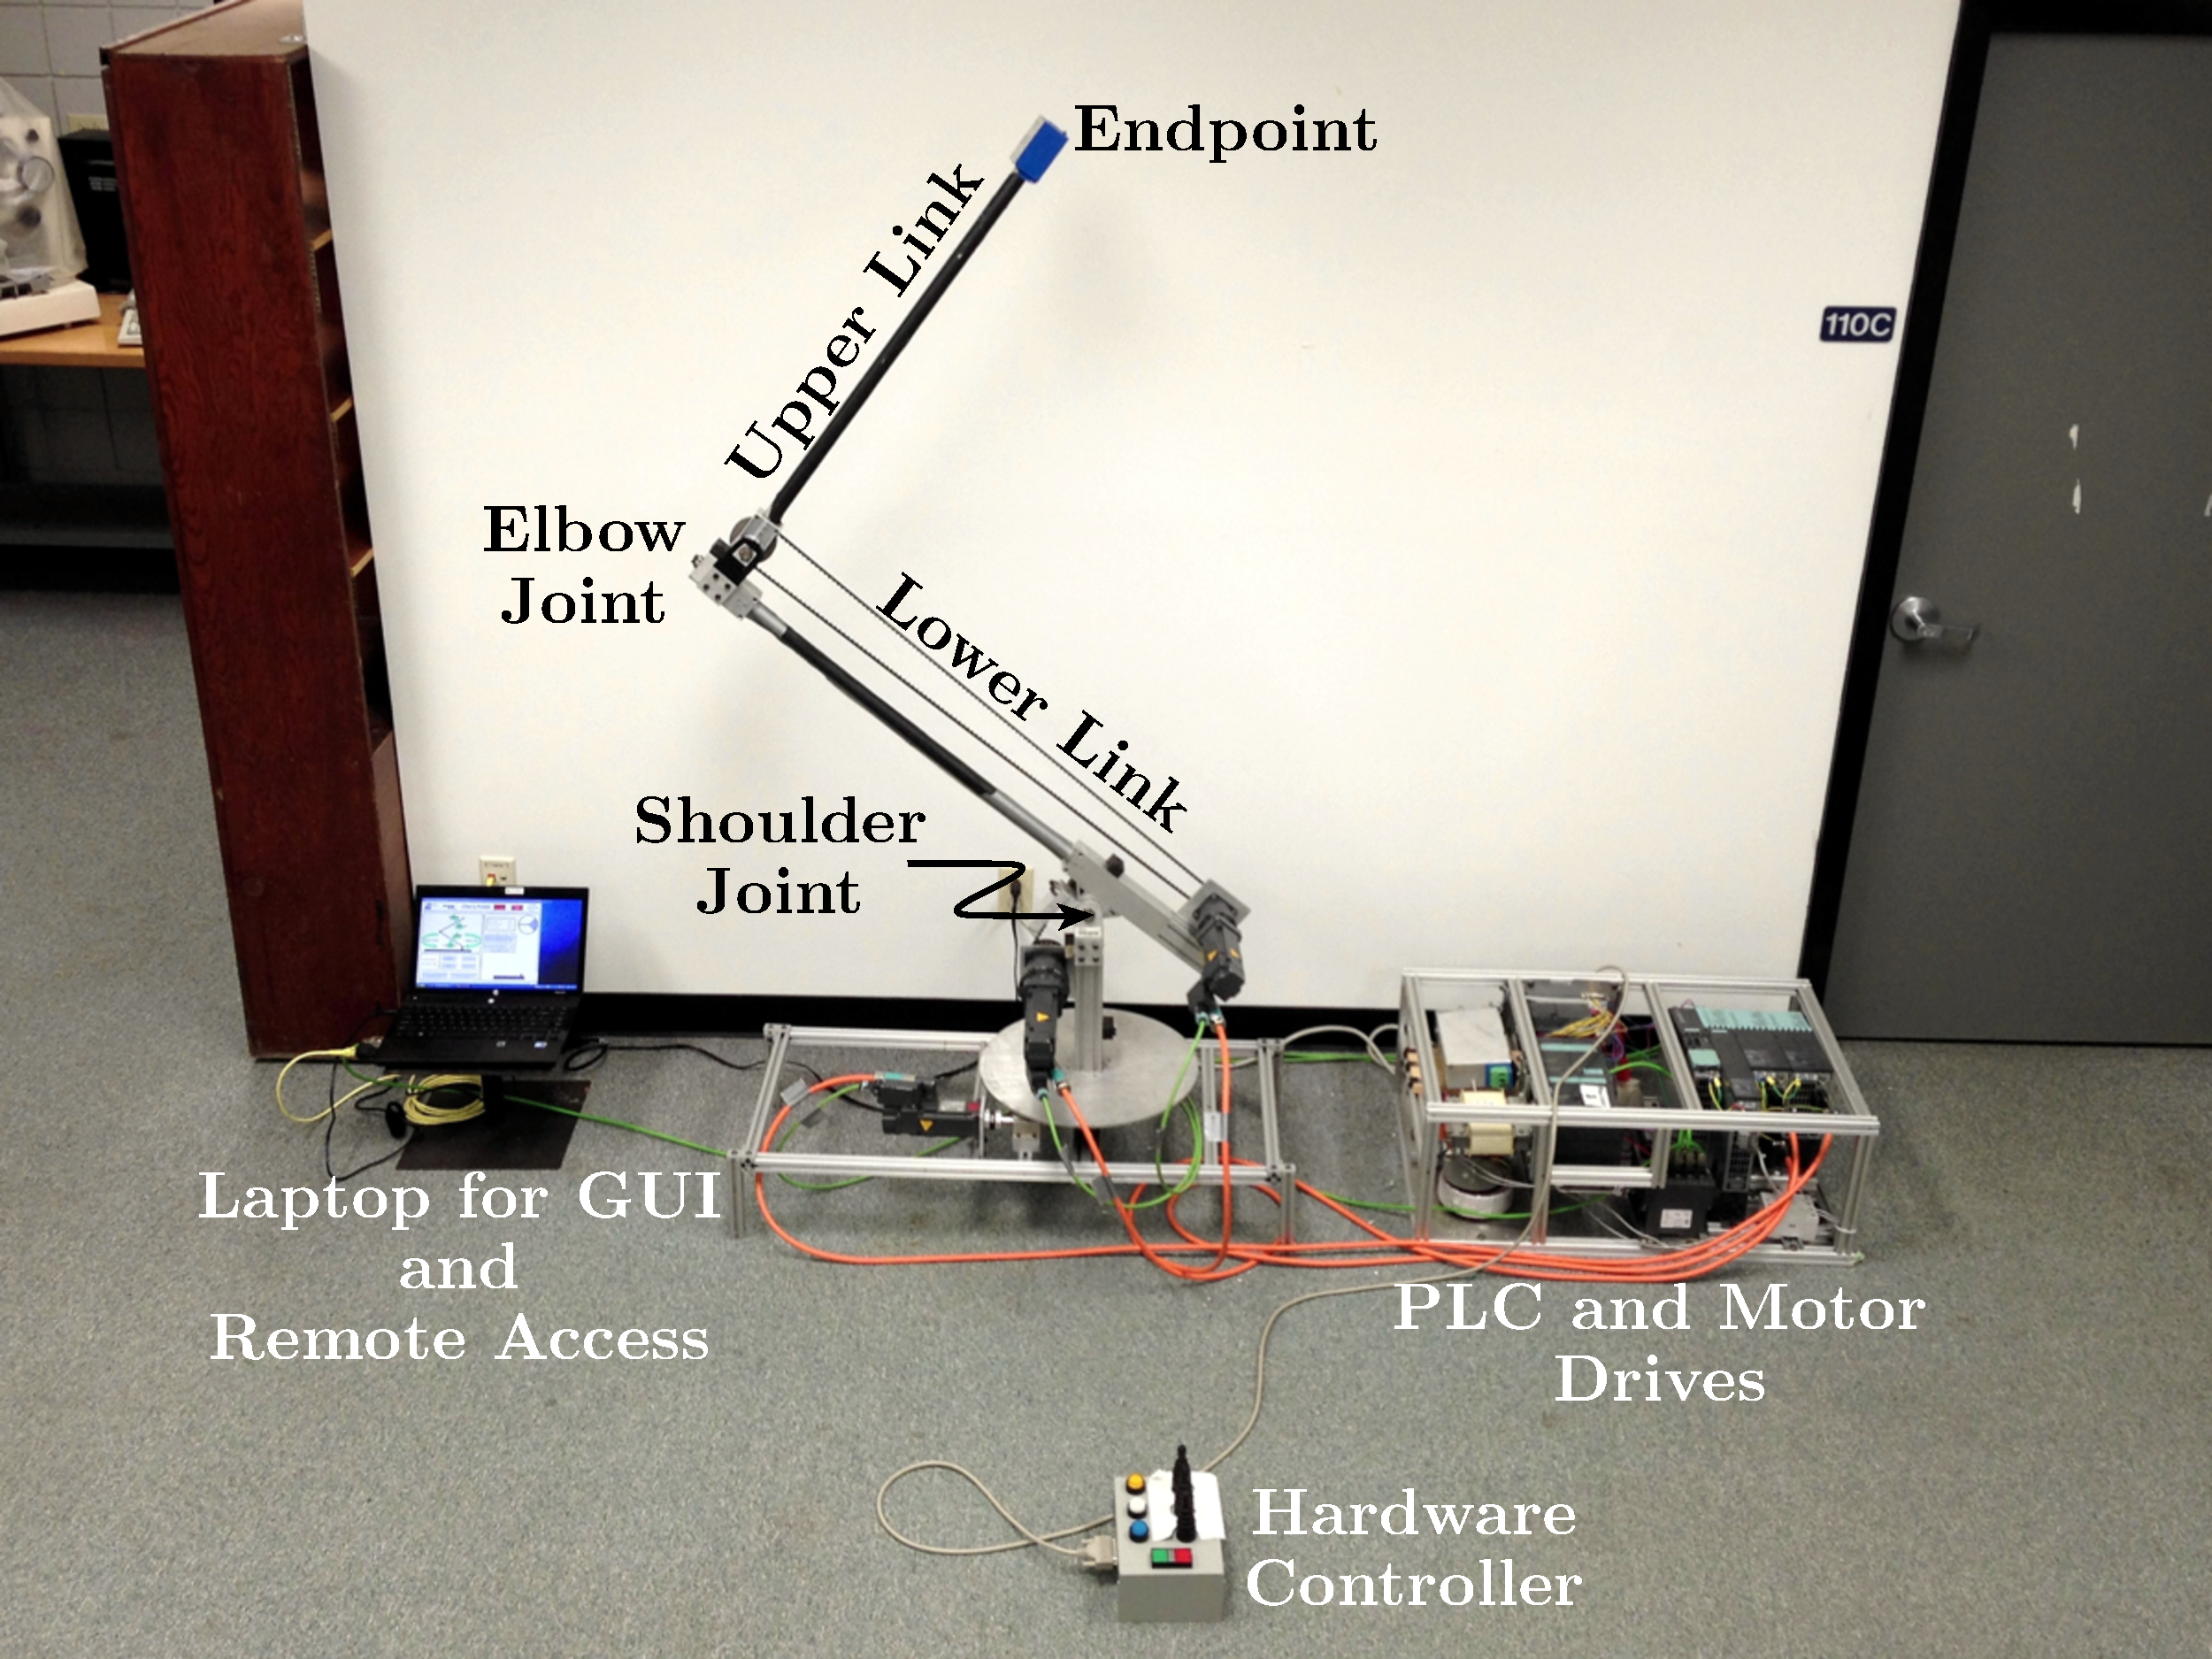
\includegraphics[width = 4in]{Cherrypicker_labeled}
\caption{The Experimental Setup}
\label{fig:cherrypicker_labeled}
\end{center}
\vspace{-0.2in}
\end{figure}
%

%%%%%%%%%%%%%%%%%%%%%%%%%%%%%%%%%%%%%%%%%%%%%%%%%%%%%%%%%%%%%%%%
\subsection{Using Tables}
\label{sec:tables}
\vspace{-0.2in}
%
A table is shown in Table \ref{table:sim_parameters}. Table captions should go above your tables. \LaTeX will handle this, along with numbering the tables in the order that they appear. There are many tools for creating \LaTeX tables, including some macros that will do so from an Excel file, or similar. 

% The code below is what creates the table.
\begin{table}
\label{table:sim_parameters}
\begin{center}
\caption{Parameters Used In Simulation}
\vspace{0.1in}
\begin{tabular}{ll}
\hline
\hline
Parameter & Value  \\
\hline
Leg Mass, $m_l$ & 0.175 kg \\
Actuator Mass, $m_a$ & 1.003 kg  \\
Natural Frequency & 11.13 Hz \\
Gravity  & 0.276g $\frac{m}{s^2}$ \\[1ex]
\hline
Stroke Length, $(x_a)_{max}$ & 4 mm \\
$(\ddot{x}_a)_{max}$ & 25 $\frac{m}{s^2}$ \\
$(\dot{x}_a)_{max}$ & 0.4 $\frac{m}{s}$ \\
\end{tabular}
\end{center}
\end{table}

%%%%%%%%%%%%%%%%%%%%%%%%%%%%%%%%%%%%%%%%%%%%%%%%%%%%%%%%%%%%%%%%
%%%%%%%%%%%%%%%%%%%%%%%%%%%%%%%%%%%%%%%%%%%%%%%%%%%%%%%%%%%%%%%%
\section{Conclusion}
\label{sec:conclusion}
\vspace{-0.2in}
%
Aliquam aliquet, est a ullamcorper condimentum, tellus nulla fringilla elit, a iaculis nulla turpis sed wisi. Fusce volutpat. Etiam sodales ante id nunc. Proin ornare dignissim lacus. Nunc porttitor nunc a sem. Sed sollicitudin velit eu magna. Aliquam erat volutpat. Vivamus ornare est non wisi. Proin vel quam. Vivamus egestas. Nunc tempor diam vehicula mauris. Nunc tempor diam vehicula mauris. Nullam sapien eros, facilisis vel, eleifend non, auctor dapibus, pede. Ut nulla. Vivamus bibendum, nulla ut congue fringilla, lorem ipsum ultricies risus, ut rutrum velit tortor vel purus.






\end{document}